\section{Results}

Here you should describe all the graphs and see similar stuff on paper you read and cite them and tell how your results are compared to that stuff.

Also add unitary event analysis

\myparagraph{PCA} 

The first novel analysis performed on the data was PCA.	Before applying it, the data has been convoluted with a gaussian kernel with $\sigma=10$, normalized using the activity of 500ms before and after the landmark, and at last averaged across trials, for the reasons explained above.
\begin{figure}[h]
	\centering
	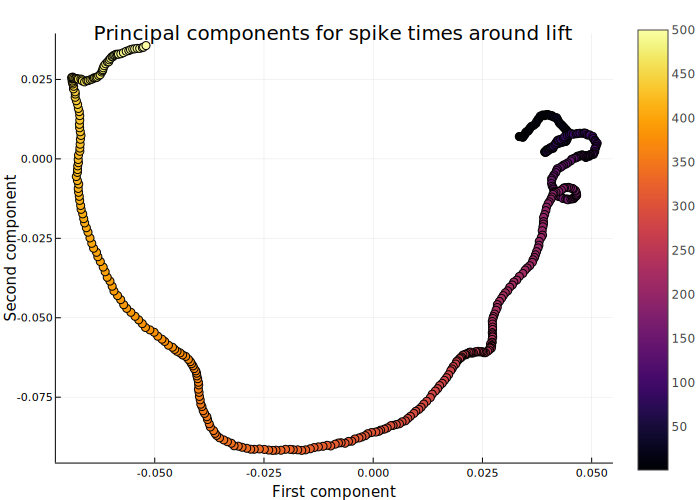
\includegraphics[scale=0.8]{../../plots/pca-500-lift.pdf}
	\caption{Trajectory of the 2 principal components of most active spike trains 250ms before and after lift. 
}
	\label{fig:pca-500}
\end{figure}

The observed trajectory represents [cit dimensionality reduction in neuroscience] how the small population of neurons recorded encodes the arm lifting. It is noticeable a circular trajectory, as it is found in the motor and premotor cortex [cit]. 

It is worth noting that this kind of trajectory is not found in if applying PCA on other time points, when the rats were not performing the same action simultaneously. For example, [figure x] shows the pattern plot between $t_l_i_f_t-1.5s$ and $t_l_i_f_t-1.0s$
\begin{figure}[h]
	\centering
	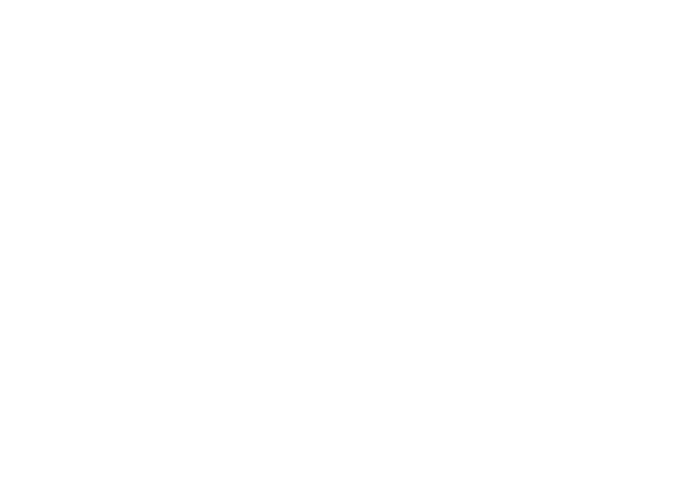
\includegraphics[scale=0.8]{../../plots/pca-500-before-lift.pdf}
	\caption{Trajectory of the 2 principal components between 1.5s and 1s before lift}
	\label{fig:pca-500-before-lift}
\end{figure}


A further step has been taken in this direction, analysing the differences in the principal components of trials were the inverval between \emph{lift} and \emph{cover} was high and were it was low, basically exploring the differences that speed has on the neural trajectory.
It is very interesting to notice that the trajectories are starting very close, but then they follow almost specular paths.

\begin{figure}[h]
	\centering
	\includegraphics[scale=0.8]{../../plots/pca-speed.pdf}
	\caption{Trajectory of the 3 principal components  between 250ms before and after lift. Trajectory of neural response of faster movements is in red, and in blue for slower movements. Light is start of trajectory, dark is end.}
	\label{fig:pca-500-before-lift}
\end{figure}

\myparagraph{Gaussian-Process Factor Analysis} 
